\documentclass{llncs}
\usepackage{epsfig,amsmath,graphicx,cite,lmodern}
\usepackage{subfig,url}
\usepackage[utf8]{inputenc}
\usepackage{verbatim}

\begin{document}
\mainmatter

\title{Eine Übersicht über Crossover-Operationen für genetische Algorithmen\\Seminar Organic Computing}
\titlerunning{Eine Übersicht über Crossover-Operationen für genetische Algorithmen}  % abbreviated title (for running head)

\author{Gerald Siegert\\Matrikelnummer: 1450117}
\authorrunning{Siegert} % abbreviated author list (for running head)
\tocauthor{}

\institute{Universität Augsburg\\Lehrstuhl für Organic Computing\\
\email{student@organic-computing.org}}

\maketitle


%-------------------------
\begin{abstract}
	Crossover-Operationen (CO) sind ein wesentlicher Teil von Genetischen Algorithmen (GA) und sind maßgeblich für deren Effizienz. Daher soll ein kleiner Überblick über verschiedene COs und deren Klassifizierung gegeben werden. Zunächst werden eindimensionale Re\-prä\-sen\-ta\-ti\-on\-en betrachtet. Dabei werden Darstellungen als Binärwerte, Ganzzahlen bzw. entsprechende Permutationen, Fließkommazahlen und Zeichenketten erläutert, bei welchen Problemen bzw. Anwendungsfällen welche Darstellung geeignet ist, und einige der dafür optimierten COs aufgezeigt. Ebenso betrachtet werden mehrdimensionale Re\-prä\-sen\-ta\-ti\-on\-en wie Bäume und Arrays. Es wird zudem eine kleine Über\-sicht über weitere mehrdimensionale Repräsentationen gegeben. Ebenso wird auch darauf eingegangen, wann es geeignet ist, anwendungsspezifische Co\-die\-rungen zu nutzen und anzuwenden. Ebenso werden zudem einige universell nutzbare COs aufgezeigt, die nicht an eine spezielle Repräsentation der Daten gebunden sind.
\end{abstract}

\pagebreak

\section{Einführung in genetische Algorithmen}
\label{sec:EinfuhrungGA}

	Genetische Algorithmen (GA) sind genauso wie andere Evolutionäre Algorithmen im Allgemeinen aus der Biologie übernommen worden. Wie der Name schon aussagt, basieren sie auf dem Prinzip der Evolution, bei der basierend auf einer Ausgangspopulation möglicher Lösungen neue Kinder erzeugt werden, welche dann die Vorfahren in der Population verdrängen. Welche Vorfahren, oder gar die erzeugten Kinder, dabei konkret verdrängt werden, entscheidet sich basierend auf einer Fitness-Funktion, bei der die gefundenen Lösungen der Population evaluiert werden und anschließend nur die besten in der Population verweilen dürfen.
	
	\begin{figure}
		\centering
		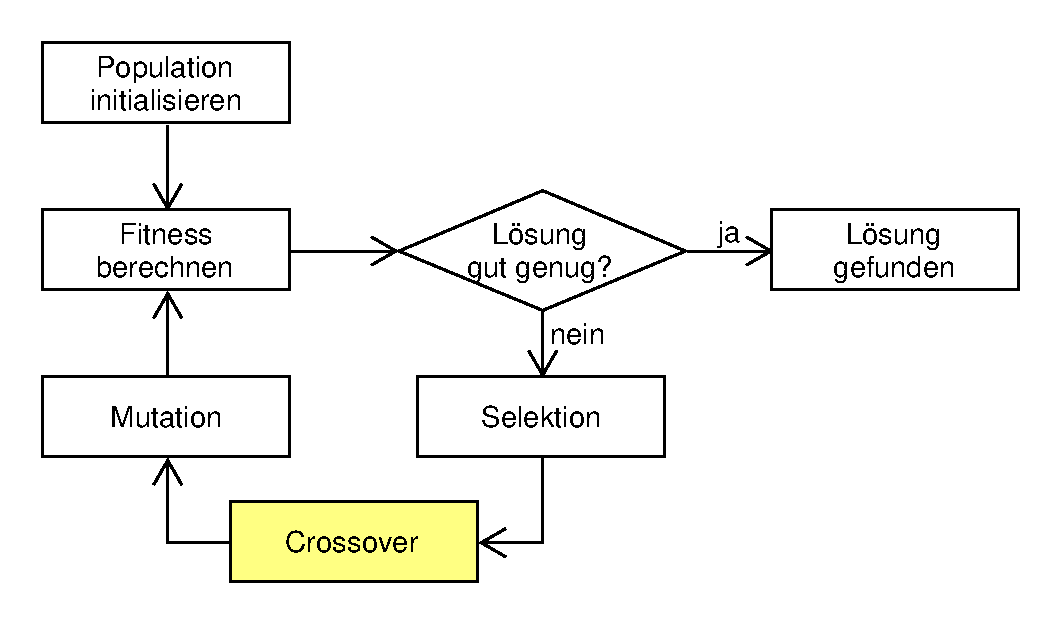
\includegraphics[width=.8\columnwidth]{./Figures/GA-Prinzip.pdf}
		\caption{Grundlegender Ablauf eines genetischen Algorithmus}
		\label{fig:abb1}
	\end{figure}	

	Die wichtigen Parameter eines GA selbst sind zum einen die Selektion der Gene, deren Crossover-Operationen (CO) zur Erzeugung neuer Kinder, sowie die Durch\-füh\-rung anschließender Mutationen. Maßgeblich für die Qualität und Effizienz eines GA ist dabei die in Fig. \ref{fig:abb1} markierte CO.
	
	In dieser Seminararbeit soll daher nun ein kleiner Überblick über einige verschiedene COs gegeben werden. Nach einer Übersicht der Klassifikationen im Abschnitt \ref{sec:KlassifizierungCrossover} werden im Abschnitt \ref{sec:EindimensionaleRep} zuerst geeignete Anwendungen und dazugehörige COs für eindimensionale, im darauf folgenden Abschnitt \ref{sec:MehrdimRep} für mehrdimensionale Repräsentationen aufgezeigt. Anschließend wird im Abschnitt \ref{sec:AnwendungsspezifischeCod} ein kurzer Überblick über anwendungsspezifische Codierung sowie im Abschnitt \ref{sec:UniversaleOp} ein Überblick über universell einsetzbare COs gegeben.

\section{Klassifizierungen von Crossover-Operationen}
\label{sec:KlassifizierungCrossover}

	\begin{figure}
		\centering
		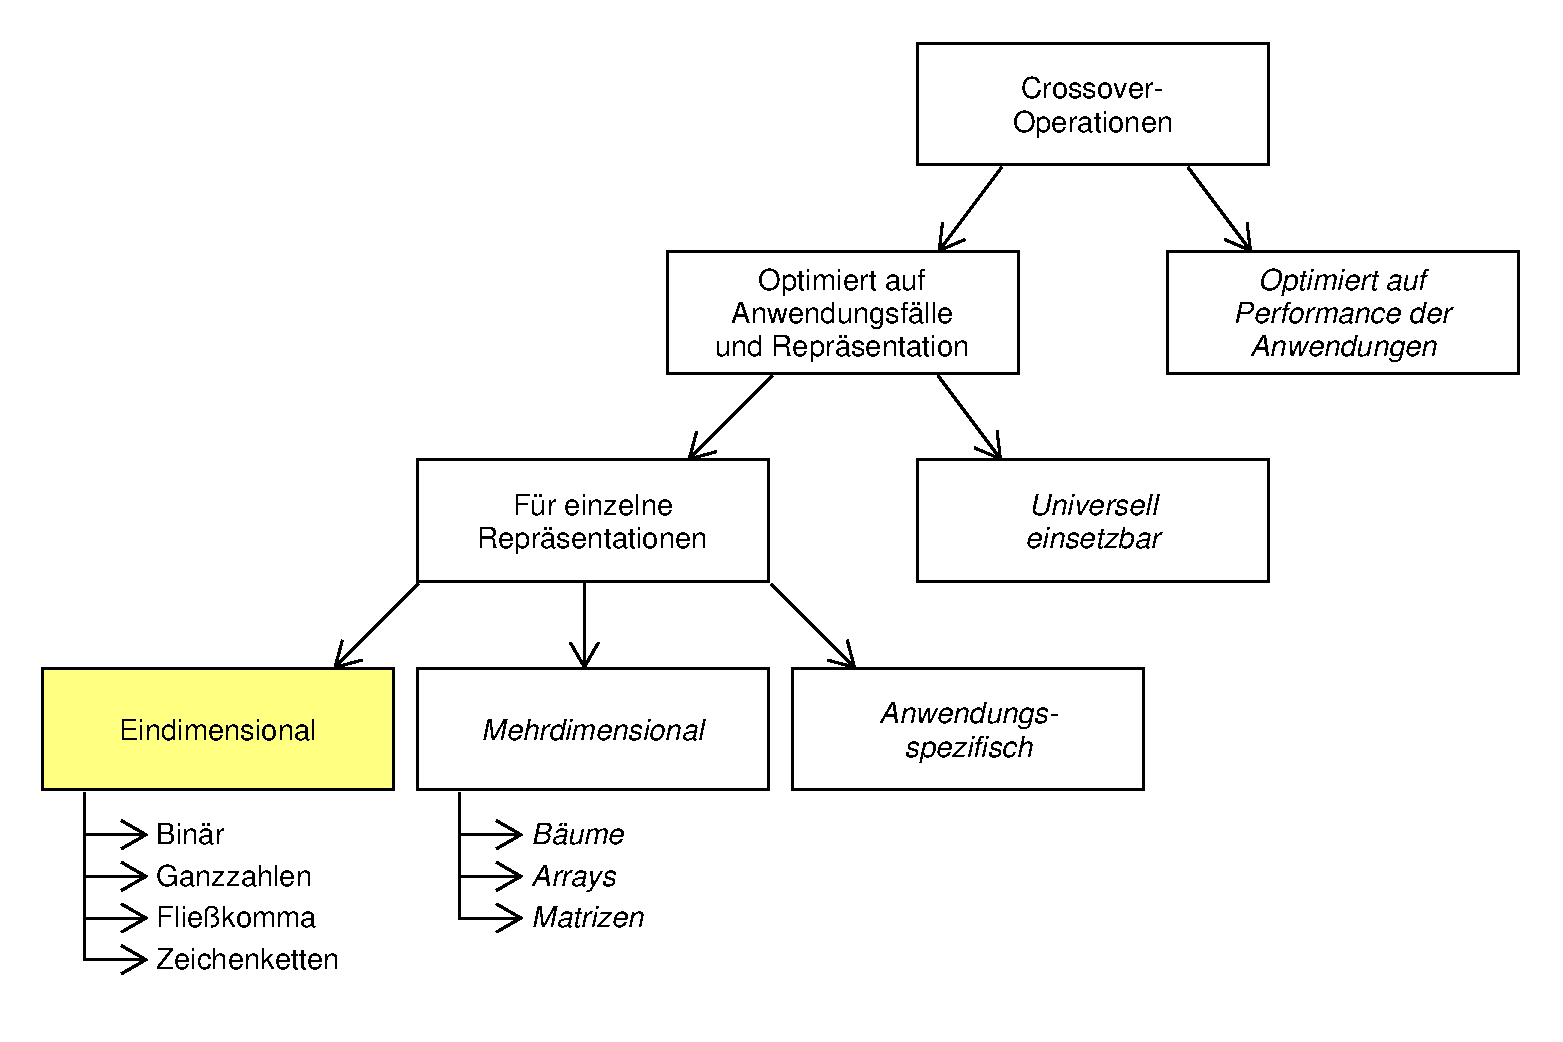
\includegraphics[width=.8\columnwidth]{./Figures/Crossover-Klassifizierung.pdf}
		\caption{Übersicht der Klassifizierung (nach \cite{Survey})}
		\label{fig:abb2}
	\end{figure}

	COs gibt es für viele verschiedene Arten von Anwendungen und Daten. Nicht alle möglichen Operationen sind jedoch für jede Anwendung und Daten anwendbar. Pavai und Geetha haben in \cite{Survey} bereits sehr gut einen Überblick über die Verschiedenen Arten von COs gegeben, weshalb sich diese Seminararbeit an deren Arbeit orientiert. COs können, wie in Fig. \ref{fig:abb2} dargestellt, in verschiedenen Kategorien klassifiziert werden. Diese Seminararbeit beschränkt sich auf die repräsentativen Darstellungsformen der Daten und deren entsprechenden COs. Für die kursiv markierten Klassifizierungen wird daher nur ein kurzer Überblick bzw. im Falle der performance-optimierten COs darauf verzichtet.

	Die Basis aller verschiedenen COs bilden die Elementaren Operationen, welche die Gene der beiden Eltern an einer oder mehreren Stellen teilen und daraus die neuen Kinder erzeugen. Entsprechend werden sie auch \textit{N-Point-Crossover} bzw. im Speziellen auch \textit{One-Point-Crossover} oder \textit{Two-Point-Crossover} genannt. Darauf basierend gibt es noch weitere Basis-Operationen, wie \textit{Segmented Cross\-over}, bei der die Gene in eine bestimmte Anzahl Segmente anstatt an einer bestimmten Anzahl an Stellen geteilt werden\cite{GABasicIdeas}, oder wie \textit{Uniform Crossover}, bei der für jede Stelle des Kindes zufällig ausgewählt wird, welcher Elternteil sein Gen vererbt.

\section{Eindimensionale Repräsentation}
\label{sec:EindimensionaleRep}

	Unter eindimensionaler Repräsentation wird vor allem die Darstellung der Daten in den elementaren Datentypen verstanden. Die Daten liegen dabei nur linear in einer bestimmten Reihenfolge vor, wodurch die Handhabung mit den Daten auch entsprechend einfach ist und in vielen Anwendungsfällen ohne große Probleme durchgeführt werden kann und entsprechend oft genutzt wird.
	
	Zuerst wird im Abschnitt \ref{sec:BinCod} ein Überblick über Anwendungsfälle und mög\-liche COs für die Binär-Codierung gegeben. Anschließend wird in Abschnitt \ref{sec:IntCod} auf ganzzahlige Codierung eingegangen, in Abschnitt \ref{sec:FloatCod} folgen Fließkomma-Darstellungen sowie in \ref{sec:StrCod} Zeichenketten.

	\subsection{Binäre Codierung}
	\label{sec:BinCod}
	
		Eine Codierung als Binärwerte bedeutet, dass die Werte, die vom GA bearbeitet werden, als eine Kette von 0 und 1 dargestellt sind. Der große Vorteil einer binären Codierung liegt vor allem darin, dass die Handhabung entsprechender Daten sehr einfach und platzsparend ist, weshalb diese Art der Darstellung prinzipiell von jeder Anwendung genutzt werden kann. Ebenfalls ein großer Vorteil liegt darin, dass entsprechende GAs aufgrund des geringen Alphabets sehr schnell und effizient sind.\cite{TacklingRealCodedGA}
		
		Vor allem folgende Arten von Anwendungen sind besonders dafür geeignet, mit binärer Codierung zu Arbeiten:\cite{Survey}
		\begin{description}
			\item[Klassifizierungs-Problem] Lösung soll in verschiedene Kategorien klassifiziert werden\cite{NearestNeighborClassifier}
			\item[\textit{Multimodal Spin Lattice}-Problem] Suchen eines minimalen Ener\-gie\-zu\-stan\-des für 450 Spins mit je vier Zuständen auf einem 2D-Gitter\cite{SelectionSchemesSpatialIsolation}
		\end{description}
		
		Passende Crossover-Operationen dafür sind:
		\begin{description}
			\item[Self-Crossover] Tauschen von einzelnen Bits innerhalb des Chromosoms\cite{SelfCrossover}
			\item[Supplementary Crossover] Nutzt das \textit{Center of Gravity}-Paradigma um Kin\-der zu erzeugen\cite{SupplementaryCrossover}
			\item[Generalized crossover] Interpretiert Chromosom als Ganzzahl und dividiert diese durch eine andere, zufällig ausgewählte Ganzzahl\cite{GeneralizedCrossover}
		\end{description}
	
	\subsection{Codierung als Ganzzahlen}
	\label{sec:IntCod}
	
		Da ganzzahlige Werte ebenfalls sehr einfach als Binärwerte dargestellt werden können, können COs für Binärwerte auch für ganzzahlige Werte eingesetzt werden. Daher wird hier vor allem auf Permutationen, also Ketten von mehreren Zahlenwerten in einer bestimmten Reihenfolge, eingegangen.
		
		Permutationen von Integer-Werten (zB TSP)
	
	\subsection{Codierung als Fließkommazahl}
	\label{sec:FloatCod}
	
		Fließkommazahlen
	
	\subsection{Codierung als Zeichenkette}
	\label{sec:StrCod}
	
		String-Codierungen

\section{Mehrdimensionale Repräsentation}
\label{sec:MehrdimRep}

	Mehrdimensionale

	\subsection{Codierung als Baum}
	\label{sec:BaumCod}
	
		Bäume und deren nutzen
	
	\subsection{Codierung als Array}
	\label{sec:ArrayCod}
	
		Array und deren Nutzen
	
	\subsection{Weitere Codierungen für mehrdimensionale Daten}
	\label{sec:WeitereMehrdimensionale}
	
		Kurz weiteres wie Matrizen und modularisierte Codierung

\section{Anwendungsspezifische Codierung der Daten}
\label{sec:AnwendungsspezifischeCod}

	Kurz anwendungsspezifisches

\section{Universale Crossover-Operationen}
\label{sec:UniversaleOp}

	Kurz auf weitere, universal einsetzbare Operationen eingehen (besser am Anfang?)

\section{Zusammenfassung und Ausblick}
\label{sec:Zusammenfassung}

	Kurze Zusammenfassung

\bibliographystyle{splncs03} 
\bibliography{literature}





\newpage

\begin{comment}
\subsection{Grundlagen}
Text zu Fig.~\ref{fig:abb1}. Siehe Formel~\ref{eq:mean}

\subsubsection{Advantages and Challenges}
Eine Subsubsection.


\begin{figure}
	\centering
	\subfloat[Beispielbild 1]{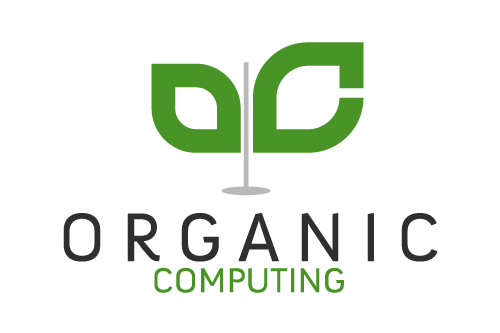
\includegraphics[width=0.5\columnwidth]{./Figures/Organic-Computing.png}}
	\hfill
	\subfloat[Beispielbild 2]{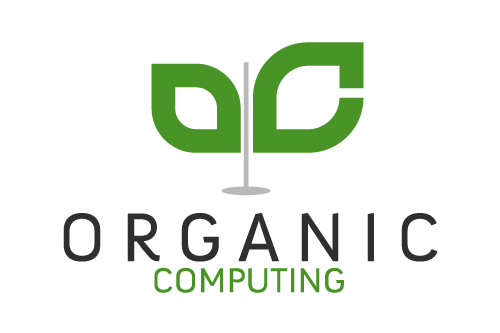
\includegraphics[width=0.5\columnwidth]{./Figures/Organic-Computing.png}}
	\caption{Zwei Beispielbilder.}
\end{figure}

\begin{equation}
\label{eq:mean}
\bar{e} = \frac{1}{N}\sum_{i=1}^N{\lvert f_i - x_i\rvert}
\end{equation}
\end{comment}

\end{document}
